\documentclass[border=1pt]{standalone}
\usepackage[dvipsnames]{xcolor}
\usepackage{amssymb}
\usepackage{tikz}                       % Graphen und kommutative Diagramme
\usetikzlibrary{patterns}               % Um schraffierte Formen in der tikzpicture-Umgebung zu zeichnen.
\usetikzlibrary{shapes}                 % Vielecke

\begin{document}

\newcommand{\ul}{\underline}
\newcommand{\A}{\mathbb A}

\newcommand{\radmult}
{
    \ensuremath{
	\tikz[baseline={([yshift=-1pt]current bounding box.center)}, x=5pt, y=2.5pt, every node/.style={shape=circle, fill=black, inner sep=.8pt}]{
	    \draw[line width=0.9pt] (5, 0) -- (3, 0);
	    \draw[line width=0.9pt] (2, 0) -- (0, 0);
	    \filldraw (3, 0) circle (1pt);
	    \filldraw (2, 0) circle (1pt);
	}
    }
}

\newcommand{\equals}
{
    \ensuremath{
	\tikz[baseline={([yshift=2pt]current bounding box.center)}, x=5pt, y=2.5pt]{
	    \node (0, 0) {$=$};
	}
    }
}

\centering
\begin{minipage}{.3\textwidth}
\centering
\resizebox{!}{3cm}{
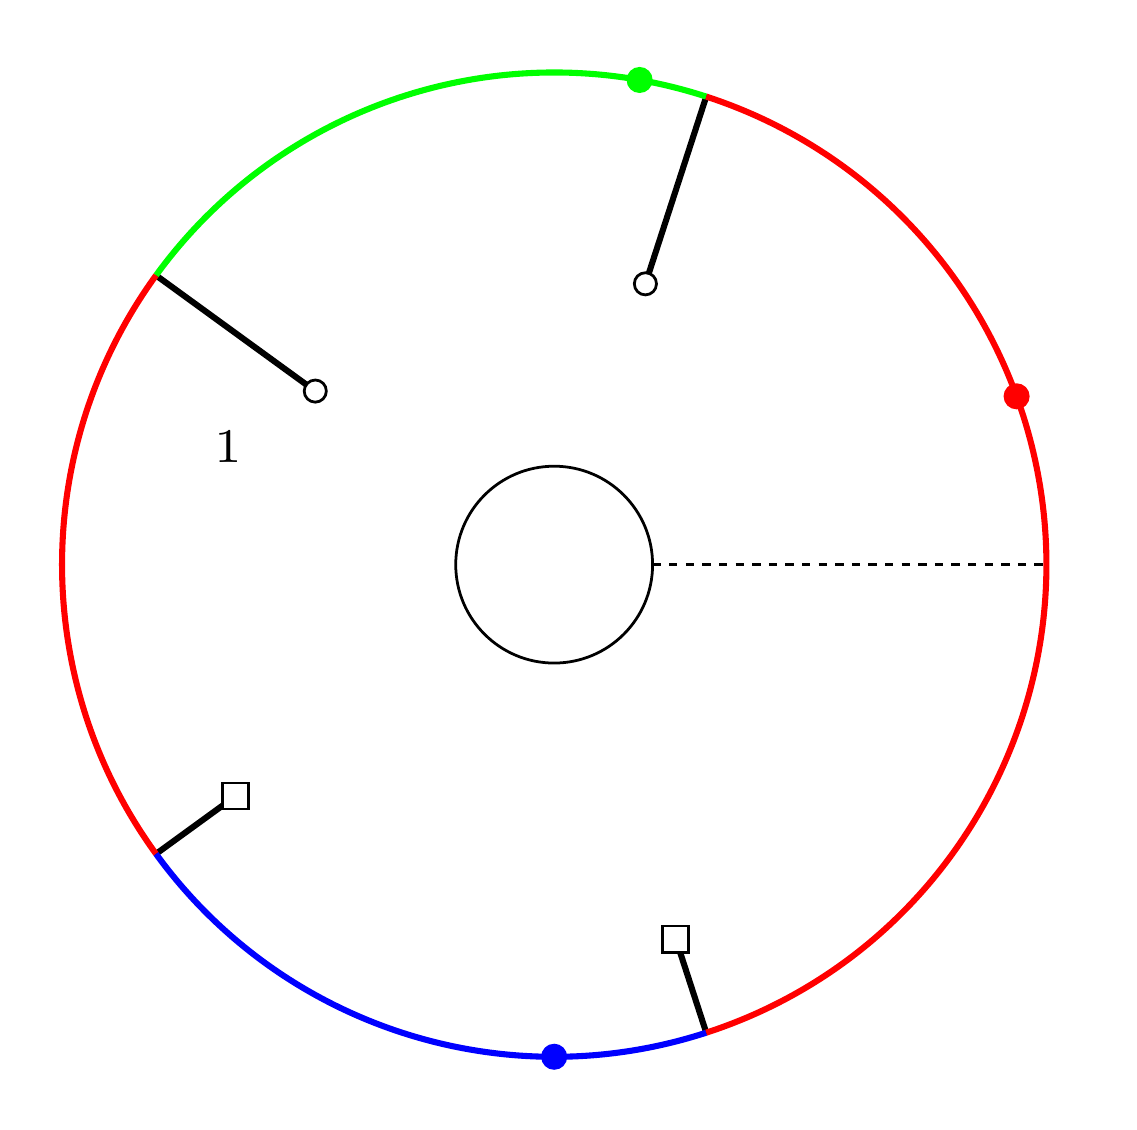
\begin{tikzpicture}[x=1.25cm, y=1.25cm, line width=1pt]
    % draw inner and outer circles
    \draw[color=black] (0, 0) circle (1);
    \draw[color=black] (0, 0) circle (5);
    
    % draw 0 line
    \draw[color=black, dashed] (0 : 1) -- (0 : 5); 
    
    % draw shaded slit box
    \draw[color=black, line width=2.2pt] (72 : 3) -- (72 : 5);
    \filldraw[color = black, fill = white] (72 : 3) circle (4pt);

    \draw[color=black, line width=2.2pt] (2 * 72 : 3) -- (2 * 72 : 5);
    \filldraw[color = black, fill = white] (2 * 72 : 3)   circle (4pt);
    
    \draw[color=black, line width=2.2pt] (3 * 72 : 4) -- (3 * 72 : 5);
    \node[draw = black, fill = white, regular polygon, regular polygon sides = 4] at (3 * 72 : 4) {};

    \draw[color=black, line width=2.2pt] (4 * 72 : 4) -- (4 * 72 : 5);
    \node[draw = black, fill = white, regular polygon, regular polygon sides = 4] at (4 * 72 : 4) {};
    
    % draw symbols
    \node[scale = 2.5, fill = white] at (160 : 3.5) {$\A_1$};

    % draw cycles
    \draw[color = green, line width = 2.2pt] (72 : 5) arc[radius = 5, start angle = 72, delta angle = 72] (2 *72 : 5);
    \draw[color = red, line width = 2.2pt] (2 * 72 : 5) arc[radius = 5, start angle = 2 * 72, delta angle = 72] (3 *72 : 5);
    \draw[color = blue, line width = 2.2pt] (3 * 72 : 5) arc[radius = 5, start angle = 3 * 72, delta angle = 72] (4 *72 : 5);
    \draw[color = red, line width = 2.2pt] (4 * 72 : 5) arc[radius = 5, start angle = 4 * 72, delta angle = 2 * 72] (72 : 5);

    % draw marked points
    \node[fill = green, circle] at (80 : 5) {};
    \node[fill = red, circle] at (20 : 5) {};
    \node[fill = blue, circle] at (270 : 5) {};
    
    \end{tikzpicture}
}
\end{minipage}


\end{document}